\documentclass[a4paper,10pt]{article}
\usepackage[utf8]{inputenc}
\usepackage[english]{babel}
\usepackage[onehalfspacing]{setspace}
\usepackage{float}
\usepackage{biblatex}   % Using reference package
\addbibresource{mybibliography.bib}

\usepackage[nottoc]{tocbibind} %Adds "References" to the table of contents
\usepackage{graphicx}
\usepackage{hyperref}
%\graphicspath{/home/trung/Pictures/} \usepackage{float}
\hypersetup{
    colorlinks=true,
    linkcolor=blue,
    filecolor=magenta,      
    urlcolor=cyan,
}
%Document title, author and date (empty)
\title{House model References}
\author{Trung Nguyen}
\date{}

%Beginning of the document
\begin{document}

\maketitle

\tableofcontents

\section{Introduction}

This document present the basic information for calculating the house model base on RC network. The specific model can be found in the references.

% ---------------------------------------------------------------------

\section{R-C Values}

Thermal purely resistive circuits and heat transfer mode is shown in table 1.
\begin{figure}[H]
	\centering
	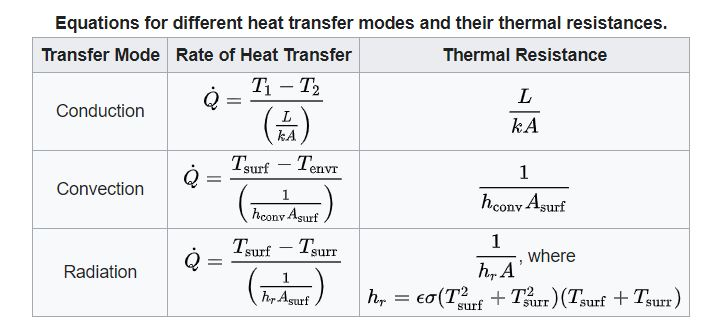
\includegraphics[width=0.8\columnwidth]{Pictures/heat transfer mode.JPG}
	\caption[Short title]{Heat transfer mode[\href{https://en.wikipedia.org/wiki/Lumped-element_model}{1}]}
	\label{table 1}
	\end{figure}
	
Some typical heat transfer resistances \href{https://www.engineeringtoolbox.com/overall-heat-transfer-coefficient-d_434.html}{[2]}: 

\begin{itemize}
    \item Static layer of air, 40 mm (1.57 in)  : R = 0.18 [$m^2K/W$].
    \item Inside heat transfer resistance, horizontal current : R = 0.13 [$m^2k/W$]. 
    \item Outside heat transfer resistance, horizontal current : R = 0.04 [$m^2K/W$].
    \item Inside heat transfer resistance, heat current from down upwards : R = 0.10 [$m^2K/W$].
    \item Outside heat transfer resistance, heat current from above downwards : R = 0.17 [$m^2K/W$].

\end{itemize}

\begin{figure}[H]
	\centering
	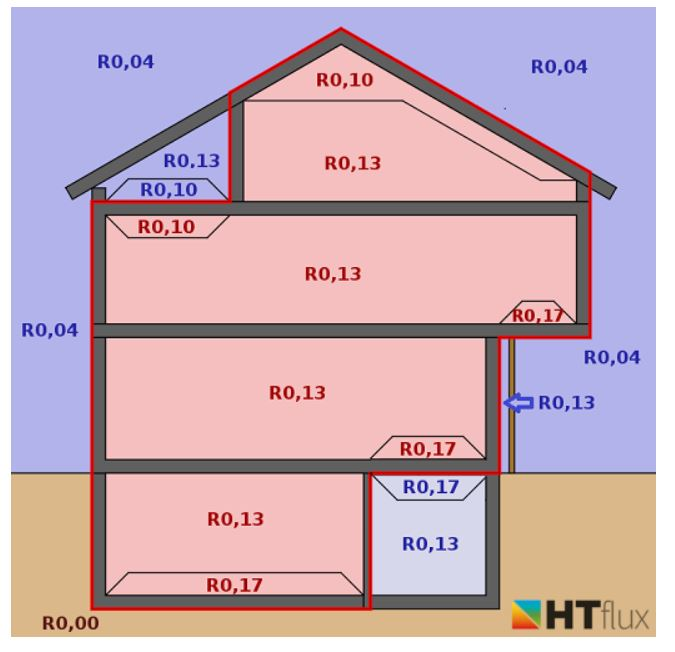
\includegraphics[width=0.8\columnwidth]{Pictures/Overview of heat resistances.JPG}
	\caption[Short title]{An overview of heat transfer resistance[\href{https://www.htflux.com/en/documentation/boundary-conditions/surface-resistance-heat-transfer-coefficient/}{3}]}
	\label{table 1}
	\end{figure}


The Rc values for facades, roof and floor standard until 2020:

\begin{figure}[H]
	\centering
	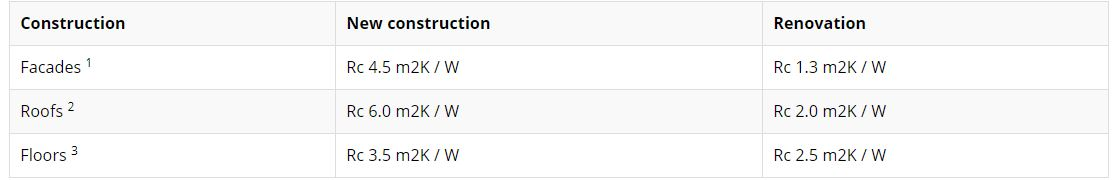
\includegraphics[width=1.2\columnwidth]{Pictures/Rc_values_2020.JPG}
	\caption[Short title]{Rc Values [\href{https://www.isolatiemateriaal.nl/kenniscentrum/het-bouwbesluit-over-isolatie-en-rc-waarde/}{4}]}
	\label{table 1}
	\end{figure}

The values will be used in 2021 has been describes in "EnergieVademecum Energiebewust ontwerpen van nieuwbouwwoningen", chapter 5: Thermische isolatie, thermische bruggen en luchtdichtheid
\href{https://v-1isso-1nl-1y6tawt2z0091.stcproxy.han.nl/q/9d67bdb7}{[5]}.

\begin{figure}[H]
	\centering
	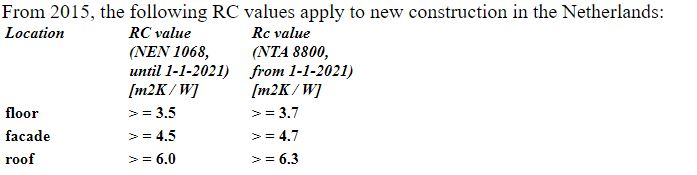
\includegraphics[width=1.0\columnwidth]{Pictures/Rc_values_2021.JPG}
	\caption[Short title]{Rc Values [\href{https://www.joostdevree.nl/shtmls/r-waarde.shtml}{6}]}
	\label{table 1}
	\end{figure}

The values used for different types of houses such as: row house, detached house, apartments ..etc can be found in "Voorbeeldwoningen 2011" \href{https://www.rvo.nl/onderwerpen/duurzaam-ondernemen/gebouwen/woningbouw/particuliere-woningen/voorbeeldwoningen}{[6]}. An example values for row house which was built from 1975 to 1991 is shown in pictures:


	
\begin{figure}[H]
	\centering
	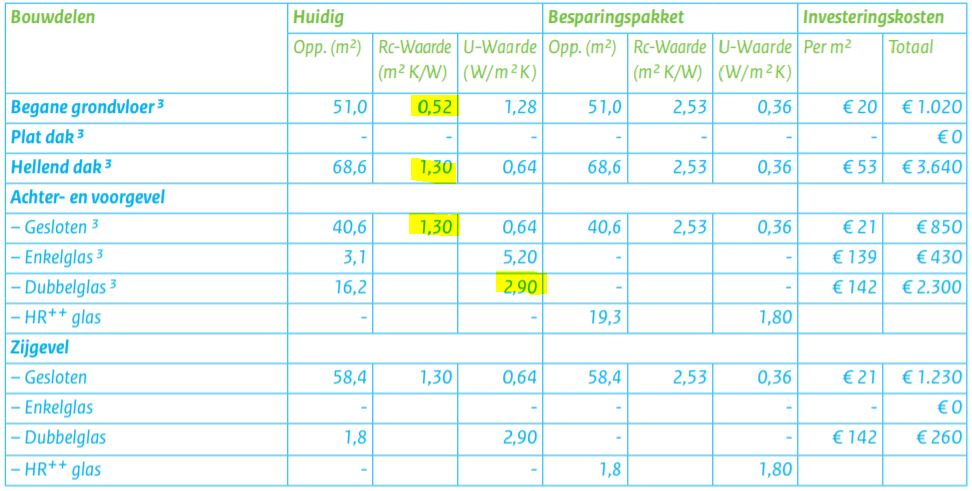
\includegraphics[width=0.8\columnwidth]{Pictures/row_house_1975-1991.JPG}
	\caption[Short title]{Rc Values for row house buit in 1975-1991 \href{Voorbeeldwoningen 2011 bestaande bouw.pdf}{[7].}}
	\label{row house}
	\end{figure} 

%----------------------------------------------------------------------

\section{NEN and ISO}

The list of NEN and ISO standard used in the calculation:

\begin{itemize}
    \item NTA 8800
    \item NEN 1068
    \item ISO 6946
    \item SO 10077-2
    \item NEN 7120
\end{itemize}

%----------------------------------------------------------------

%Bibliographic references
\begin{thebibliography}{9}

%______________________

\bibitem{1} 
\href{https://en.wikipedia.org/wiki/Lumped-element_model}{Lumped-element model}
%______________________

\bibitem{2} 
\href{https://www.engineeringtoolbox.com/overall-heat-transfer-coefficient-d_434.html}{Overall Heat Transfer Coefficient}

%______________________

\bibitem{3} 
\href{https://www.htflux.com/en/documentation/boundary-conditions/surface-resistance-heat-transfer-coefficient/}{Heat transfer resistance / surface resistance}

%______________________

\bibitem{4} 
\href{https://www.isolatiemateriaal.nl/kenniscentrum/het-bouwbesluit-over-isolatie-en-rc-waarde/}{Het bouwbesluit over isolatie en de Rc-waarde}

%______________________

\bibitem{5} 
\href{https://v-1isso-1nl-1y6tawt2z0091.stcproxy.han.nl/q/9d67bdb7/}{EnergieVademecum Energy-conscious design of new-build homes}

%______________________

\bibitem{6} 
\href{https://www.joostdevree.nl/shtmls/r-waarde.shtml}{R-waarde}

%______________________

\bibitem{7} Voorbeeldwoningen 2011 bestaande bouw

%______________________

\bibitem{8} 
\href{https://www.engineeringtoolbox.com/heat-loss-transmission-d_748.html}{Transmission Heat Loss through Building Elements}

%______________________

\bibitem{9} 
\href{https://www.e-education.psu.edu/egee102/node/2019}{Solar Heat Gain Coefficient}

%______________________

%\bibitem{10} 
%\href{https://www.isover.nl/producten/mupan-facade}{R-waarde}

\end{thebibliography}

\end{document}
